\chapter{Propuesta de solución}\label{chapter:proposal}

Este capítulo introduce la propuesta desarrollada para enfrentar el reto de clasificar de manera automática el cáncer de piel, empleando técnicas de aprendizaje profundo. La solución se centra en la utilización de una red neuronal profunda pre-entrenada, combinada con un algoritmo propio para el ajuste de precisión.

En el núcleo de nuestra estrategia se encuentra el uso de una red neuronal convolucional pre-entrenada llamada \textit{EfficientNetB1}. Esta red, desarrollada a partir de extensos conjuntos de datos y experiencias previas, ofrece una base sólida y rica en características para nuestro modelo. Al aprovechar este pre-entrenamiento, se puede acelerar significativamente el proceso de aprendizaje del modelo, al tiempo que aumentamos su capacidad para generalizar y reconocer patrones complejos en las imágenes dermatoscópicas.

Para complementar el enfoque metodológico, se seleccionan un conjunto de herramientas tecnológicas avanzadas. Estas herramientas están diseñadas para optimizar el rendimiento del modelo, mejorar la precisión de la clasificación y garantizar una implementación efectiva. Entre ellas, destaca una capa de normalización, una capa densa, una de regularización, una de \textit{dropout} y una de salida (capa densa con activación \textit{softmax}). Estas técnicas le permiten al modelo afinar su capacidad de identificar con precisión las diferentes categorías de lesiones cutáneas.

Para la optimización del algoritmo además se llevaron a cabo una serie de experimentos de los que se detallan al final de este capítulo los 2 más relevantes. Estos experimentos se realizaron con el objetivo de encontrar la mejor configuración de datos para el modelo, que permita obtener la mayor precisión posible. Para esto se utilizaron dos técnicas de normalización de datos: division asimétrica con utilización de pesos por clases y estratificación de datos. Además, se generaron distintas distribuciones de datos para los diferentes acercamientos.

Con la intensión de evaluar la efectividad y precisión del modelo se hizo uso del conjunto de datos mencionado previamente: HAM1000. Este, con más de 10000 imágenes, representa una variedad de condiciones de la piel, lo que lo convierte en un recurso valioso para entrenar y evaluar algoritmos de detección de cáncer de piel. Para esto se importan, modelan y dividen los datos para asegurar un aprendizaje efectivo

La sección que sigue detalla la metodología empleada en la preparación y carga de los datos. Esta fase es esencial, ya que la calidad y el tratamiento de los datos tienen un impacto directo en la eficacia del modelo.

\begin{figure}[ht]%
   \begin{center}
   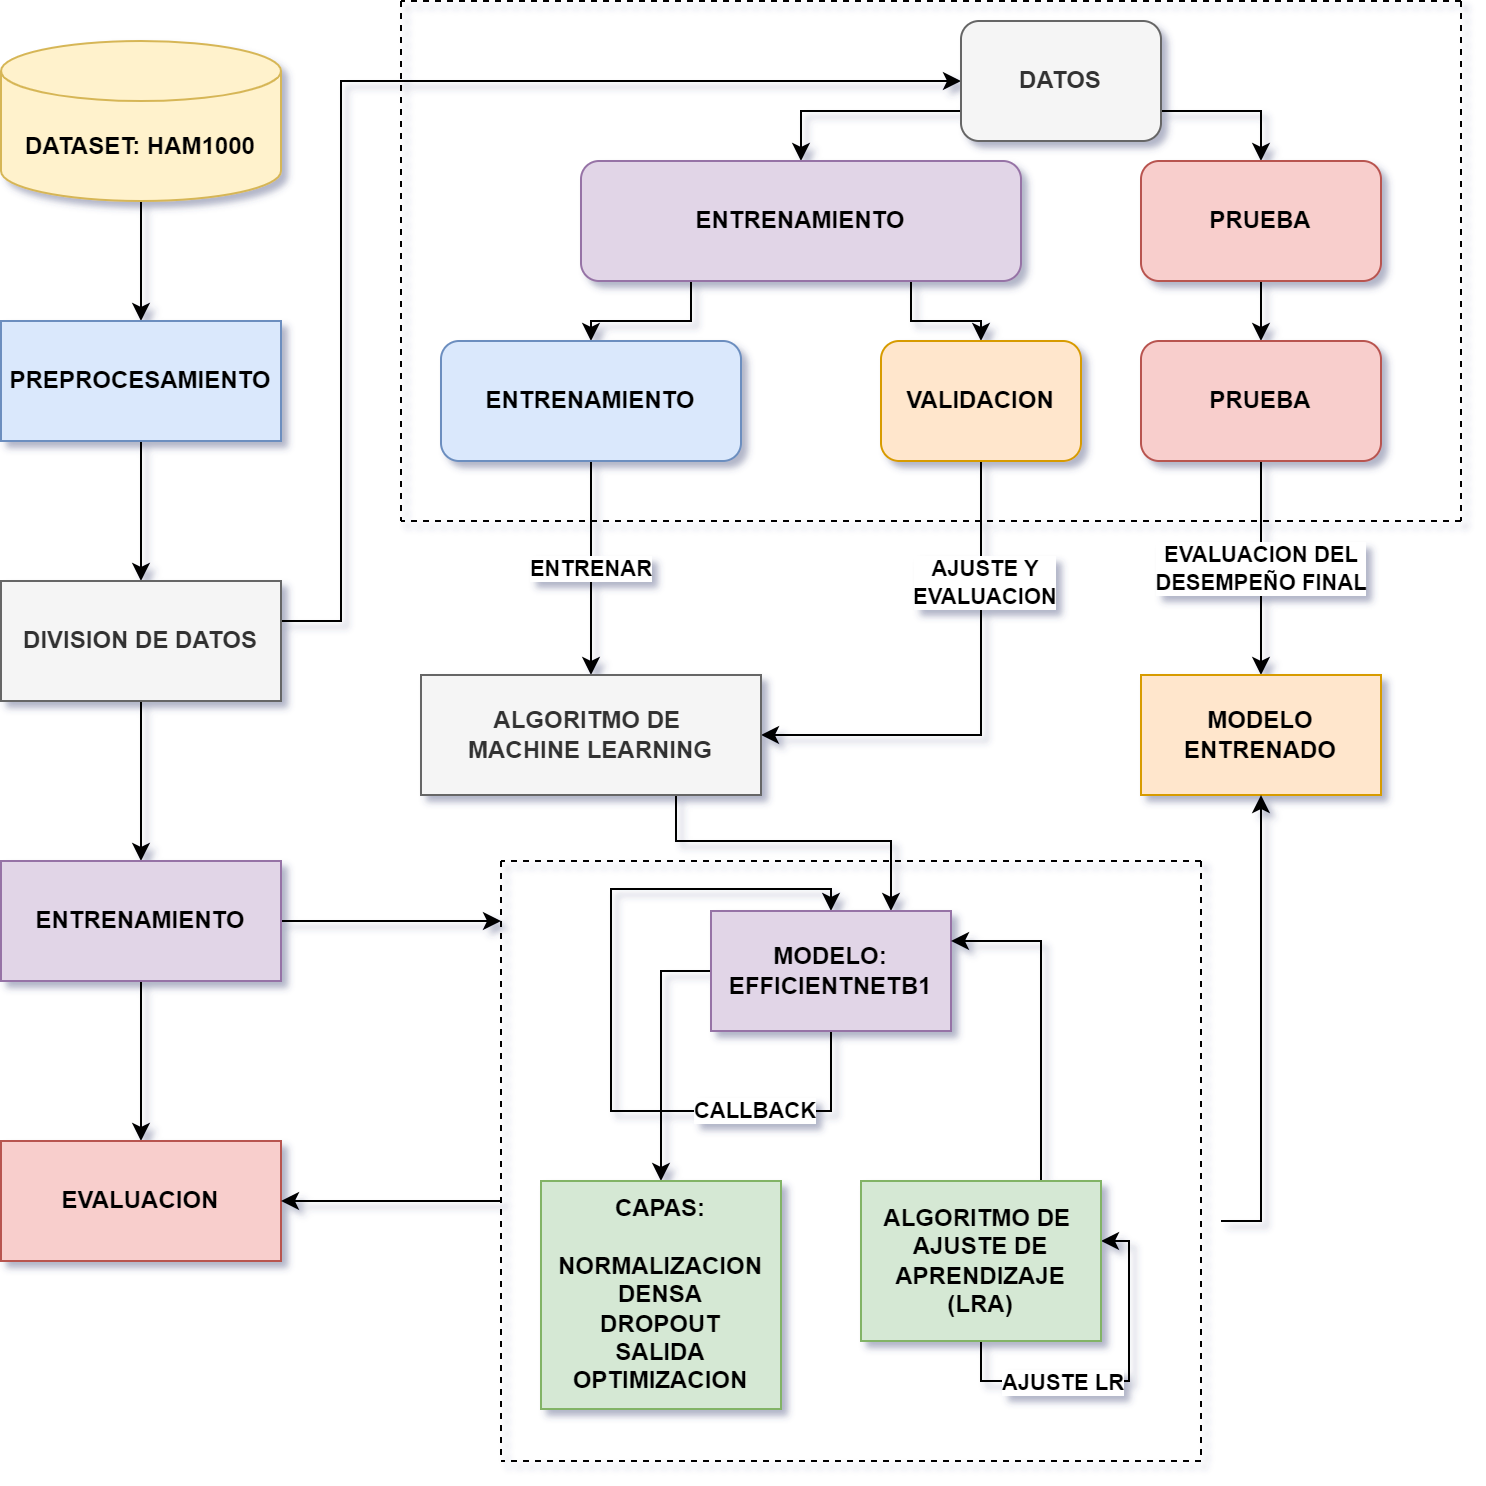
\includegraphics[width=1\textwidth]{./Graphics/model.png}
   \caption{Diagrama de flujo del proceso de entrenamiento  y validación del modelo.}
   \label{fig:model_structure}
   \end{center}
   \end{figure}

\section{Preparación y carga de datos}

En la presente sección, se describe cómo se seleccionó y procesó el conjunto HAM10000. Se detallan técnicas aplicadas para optimizar el rendimiento del algoritmo incluyendo el procesamiento de las imágenes y la conversión de los metadatos a un formato categórico adecuado para su análisis.

Posteriormente, se explica la modelación y división del conjunto de datos, utilizando herramientas como Pandas para estructurar los datos y dividirlos en conjuntos de entrenamiento, validación y prueba. Finalmente, se aborda el desafío del desequilibrio en la representación de las clases dentro del \textit{dataset}. Se detallan las estrategias implementadas para equilibrar el conjunto de datos, garantizando así que el modelo aprenda de manera efectiva a identificar una variedad de lesiones cutáneas sin sesgos hacia las condiciones más comunes.

\subsection{Dataset}

El conjunto de datos HAM10000, acrónimo de \textit{Human Against Machine with 10000 training images} (Humano Contra Máquina con 10000 imágenes de entrenamiento), se presenta como una solución al problema de la falta de diversidad y tamaño reducido en los conjuntos de datos disponibles para el diagnóstico automatizado de lesiones cutáneas pigmentadas. Este conjunto de datos es notable por su extenso alcance y diversidad, abarcando una amplia gama de lesiones cutáneas pigmentadas comunes \brackcite{tschandl2018ham10000}. 

\subsubsection*{HAM10000}

Las $10015$ imágenes dermatoscópicas del conjunto de datos HAM10000 se recopilaron a lo largo de 20 años desde dos ubicaciones diferentes: el Departamento de Dermatología de la Universidad Médica de Viena, Austria, y la práctica de cáncer de piel de Cliff Rosendahl en Queensland, Australia \brackcite{tschandl2018ham10000}. En comparación con otros conjuntos de datos, HAM10000 ofrece un conjunto más diverso y completo de imágenes dermatoscópicas para la investigación del aprendizaje automático. Las imágenes y los metadatos del HAM10000  tienen la siguiente distribución.

\begin{table}[ht]
   \centering
   \small
   \begin{tabular}{lccc}
   \hline
   \textbf{Categoría Diagnóstica} & \textbf{Cantidad} & \textbf{Porcentaje} \\
   \hline
   Melanocytic nevi (NV) & 6705 & 66.95\%  \\
   Melanoma (MEL) & 1113 & 11.11\% \\
   Benign keratosis-like lesions (BKL) & 1099 & 10.97\% \\
   Basal cell carcinoma (BCC) & 514 & 5.13\% \\
   Actinic Keratosis and Intraepithelial Carcinoma (AKIEC) & 327                         & 3.27\%              \\
   Vascular lesions (VASC) & 142 & 1.42\%  \\
   Dermatofibroma  (DF) & 115 & 1.15\% \\
   \hline
   \end{tabular}
   \caption{Distribución de imágenes por categoría diagnóstica.}
   \label{tab:ham10000_distribution}
\end{table}   
   
Las imágenes almacenadas, originalmente como diapositivas, fueron digitalizadas usando un escáner \textit{Nikon Coolscan 5000 ED}. Posteriormente, se ajustaron manualmente para centrar las lesiones y se aplicaron correcciones al histograma para mejorar el contraste visual y la reproducción del color. Para separar eficientemente las imágenes dermatoscópicas de otros tipos de imágenes (como primeros planos y vistas generales), se utilizó un método automatizado que clasificaba más de 30,000 imágenes. Se empleó una arquitectura \textit{InceptionV3}, entrenada con un conjunto de imágenes etiquetadas manualmente, para categorizar las imágenes. Las imágenes mal clasificadas por este método fueron revisadas y corregidas manualmente.  Se realizó una revisión manual final para excluir imágenes con ciertos atributos no deseados, como contenido potencialmente identificable, imágenes fuera de enfoque o con artefactos perturbadores como prendas, y lesiones completamente no pigmentadas. Las imágenes restantes fueron revisadas para asegurar una reproducción de color y luminosidad adecuadas, aplicando correcciones manuales si era necesario \brackcite{tschandl2018ham10000}. 


Los datos utilizados como medio de aprendizaje para este proyecto son imágenes y metadatos. El dataset HAM10000 contiene imágenes y un archivo de metadatos que contienen información relacionada con cada imagen en formato \textit{one hot encoding} \brackcite{ohe}.

\subsection{Transformación de datos}

Los metadatos asociados a la clasificación, etiquetados con el método mencionado (\textit{one hot encoding}), fueron convertidos a un formato \textit{categórico} \brackcite{vitalflux_categorical_crossentropy} para su procesamiento. En este proceso a cada elemento se le asignó una etiqueta basada en las categoría de la lesion cutánea, como 'MEL' (Melanoma), 'NV' (Nevus Melanocítico), entre otras. Se elimina del \textit{dataframe}, además, cualquier columna innecesaria, dejando solo las etiquetas y nombres de imágenes relevantes. De tal forma que los datos quedan distribuidos por clase.

\begin{table}[ht]
   \centering
   \begin{tabular}{lccc}
   \hline
   \textbf{index} & \textbf{Imágenes} & \textbf{Etiqueta} \\
   \hline
      0 & $ISIC\_0024306.jpg$ & NV \\
      1 & $ISIC\_0024307.jpg$ & NV \\
      2 & $ISIC\_0024308.jpg$ & NV \\
      3 & $ISIC\_0024309.jpg$ & NV \\
      4 & $ISIC\_0024310.jpg$ & MEL \\
   \hline
   \end{tabular}
   \caption{Datos transformados a formato categórico.}
   \label{}
\end{table}   

\subsection{Modelación y división del conjunto de datos}

Los datos se modelan a partir de un \textit{dataframe} de Pandas \brackcite{pandas}. Estos son divididos en 3 conjuntos: Entrenamiento, Validación y Prueba, utilizando un enfoque simple de division de datos en porcentaje. Estas divisiones son necesarias para que el modelo pueda aprender y ser evaluado correctamente.

Inicialmente, el conjunto de datos, fue dividido en dos subconjuntos: \textit{train}, que se destinó para el entrenamiento, y \textit{dummy}, que fue utilizado como una combinación temporal para los conjuntos de validación y prueba. Luego el segundo conjunto fue separado en \textit{valid}, destinado a la validación y \textit{test}, utilizado para las pruebas.

\subsection{Generadores de datos y preprocesamiento}

Uno de los principales problemas del \textit{dataset}, como se puede observar en la tabla 2.1, es el desequilibrio en la representación de las clases, un problema habitual en los conjuntos de datos médicos en los que algunas enfermedades son más raras que otras. Para solucionar este problema, el conjunto de datos se equilibra limitando el número máximo de muestras por clase. Esto garantiza que el modelo no esté sesgado hacia las clases más comunes y pueda generalizar mejor entre varios tipos de lesiones cutáneas. 

La cantidad de muestras por clase se ajustó de manera selectiva. Incluso con estas transformaciones algunas clases seguían desbalanceadas, lo que llevó a la implementación de la técnica de \textit{class weighting} \brackcite{analyticsvidhya2020classweight}. Con este método se asignó pesos diferenciados a cada clase durante el entrenamiento del modelo, reforzando así la señal de aprendizaje para las clases menos representadas.

Además, a los conjuntos segmentados en entrenamiento, validación y prueba, se les aplicó \textit{data augmentation}. Esta técnica aplicó varias transformaciones a las imágenes, como rotación, desplazamiento y zoom, durante su carga, generando lotes de imágenes optimizados para el entrenamiento y evaluación del modelo \brackcite{augmentation}.

\section{Desarrollo del modelo y estrategias de optimización}\label{sec:method}
%-----------------------------------------------------------------------------------

Para abordar efectivamente el desafío de la detección de cáncer de piel, se seleccionó la arquitectura \textit{EfficientNetB1} \brackcite{efficientnet} como base del modelo. Esta red neuronal convolucional, parte de la familia EfficientNet, se caracteriza por su alta eficiencia y precisión. Utilizando un modelo pre-entrenado, se aprovecharon los pesos derivados de conjuntos de datos extensos, lo que facilitó la adaptación del modelo a nuestro conjunto de datos específico (HAM10000) \brackcite{tan2019efficientnet}.

\subsection{Diseño y entrenamiento del modelo}

El modelo \textit{EfficientNetB1} se carga pre-entrenado con pesos de \textit{ImageNet} \brackcite{Pinecone2021ImageNet}, una amplia base de datos de imágenes ampliamente utilizada para entrenamiento y \textit{benchmarking} en visión por computadora. Luego a este se le omitió la capa superior. Al omitir la capa superior del modelo, se permite la incorporación y personalización de capas adicionales que se mencionan más adelante en el capítulo. Además, la salida del modelo base se somete a una serie de transformaciones, incluyendo normalización por lotes, capas densas con regularizaciones, y técnicas de \textit{Dropout} para prevenir el sobre-ajuste, culminando en una capa de salida optimizada para la clasificación.

\subsubsection{Arquitectura del modelo EfficientNet}
   
La familia de arquitecturas EfficientNet \brackcite{tan2019efficientnet}, surgió con el objetivo de hallar un método adecuado para escalar las CNNs de manera que mejoraran tanto en precisión (i.e., rendimiento del modelo) como en eficiencia (es decir, en términos de parámetros del modelo y FLOPS). 

Inicialmente, el enfoque se centraba en aumentar la profundidad o el ancho de la red. Sin embargo, este método de escalado único tenía limitaciones y no se comprendía completamente. La investigación de EfficientNet reveló que un escalado uniforme en todas las dimensiones de la red (profundidad, ancho y resolución) usando un conjunto de coeficientes de escalado fijos podría lograr un mejor equilibrio y rendimiento. Este enfoque innovador, denominado escalado compuesto, aborda el problema del escalado en ConvNets de manera integral. Los resultados empíricos mostraron que escalar cualquier dimensión de la red mejora la precisión, pero el beneficio disminuye en modelos más grandes. Por lo tanto, se propuso un método de escalado que coordina y equilibra estas dimensiones, en lugar de escalar una sola dimensión a la vez.

EfficientNet comenzó con la creación de un modelo base, EfficientNet-B0, utilizando una búsqueda de arquitectura neural multiobjetivo que optimizaba tanto la precisión como los FLOPS. Esta red base se caracterizaba por su bloque principal, el cuello de botella móvil invertido MBConv, y la optimización de compresión y excitación. El proceso de escalado de EfficientNet se realizó en dos etapas principales. Primero, se fijaron ciertos parámetros y luego se escaló la red base para obtener variantes más grandes, desde EfficientNet-B1 hasta B7, utilizando el método de escalado compuesto. Mientras que la arquitectura EfficientNet B0 tiene $5.3$ millones de parámetros y acepta imágenes de entrada de $224x224$, EfficientNet B7 cuenta con $66$ millones de parámetros y acepta imágenes de $600x600$ \brackcite{Tan2019EfficientNetRM}.
  
   \begin{figure}[ht]%
      \begin{center}
      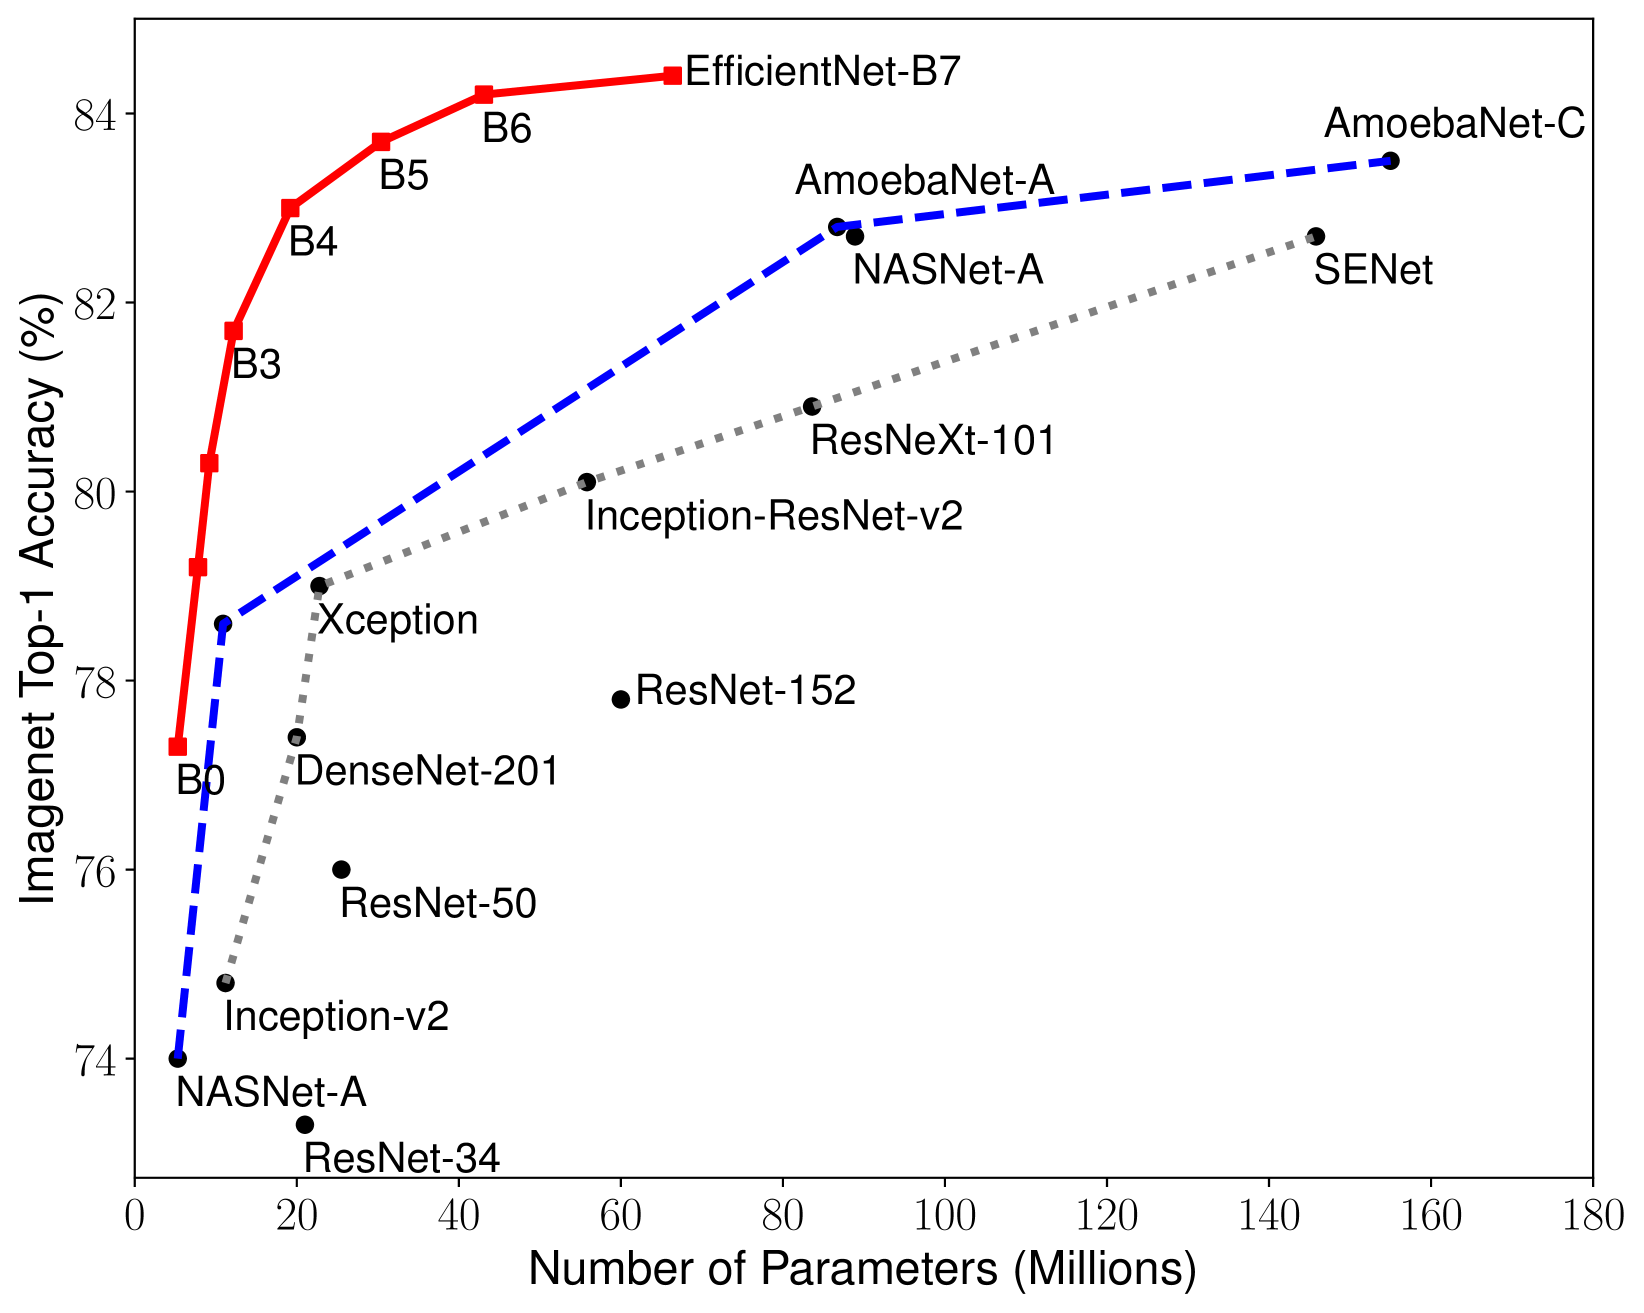
\includegraphics[width=1\textwidth]{./Graphics/efficientnet_performance.png}
      \caption{Estadísticas del rendimiento de los modelos de EfficientNet \brackcite{tan2019efficientnet}.}
      \label{fig:efficientnet_performance}
      \end{center}
      \end{figure}

Los experimentos demostraron que el método de escalado compuesto mejoraba la precisión en modelos ya existentes como MobileNets y ResNet. Los modelos EfficientNet entrenados en ImageNet mostraron una precisión y eficiencia significativamente mayores en comparación con otros ConvNets, utilizando una cantidad mucho menor de parámetros y FLOPS. Especialmente, EfficientNet-B7 logró una precisión del 84.3\% en top-1 en ImageNet, superando modelos anteriores y siendo considerablemente más pequeño y rápido.

En relación con el dataset HAM1000 \brackcite{ham10000}, la implementación del EfficientNetB1 puede ser particularmente beneficiosa para el análisis de datos. EfficientNetB1, entre las variantes de la serie EfficientNet, se encuentra en un punto medio en términos de complejidad y tamaño, ofreciendo un equilibrio entre precisión y eficiencia computacional. Dado que el HAM1000 es un conjunto de datos de imágenes dermatoscópicas que requiere una alta precisión en la identificación y clasificación de lesiones cutáneas, la utilización de EfficientNetB1 podría proporcionar una precisión y eficiencia aceptable en términos de recursos computacionales.

\subsection{Arquitectura del modelo y regularización}

Para fortalecer la arquitectura del modelo, se añadieron capas adicionales, incluyendo \textit{Dropout} y regularizadores L1 y L2, esenciales para combatir el sobre-ajuste. Una capa densa personalizada fue incorporada para facilitar la clasificación precisa de múltiples tipos de tumores. La compilación del modelo se realizó con un enfoque en la clasificación multi-clase, utilizando la pérdida de entropía cruzada categórica (\textit{categorical crossentropy}) y un optimizador \textit{Adamax}.

\subsection{Ajuste dinámico del learning rate}

Un elemento innovador del entrenamiento fue el uso de un \textit{callback} personalizado para el ajuste dinámico del learning rate \brackcite{lr}. Se implementa un mecanismo de ajuste de la tasa de aprendizaje (LRA) personalizado de Keras. Este, ajusta dinámicamente la tasa de aprendizaje durante el entrenamiento basado en la precisión y la pérdida de validación, con el objetivo de mejorar la eficiencia del entrenamiento y alcanzar una mejor convergencia. Los componentes clave del LRA son:

\begin{enumerate}
   \item Modelo: La red neuronal sobre la que se aplicará el \textit{callback}.
   \item Paciencia: El número de épocas que se esperará sin mejora en la métrica de rendimiento antes de realizar un ajuste.
   \item Umbral (\textit{Threshold}): Un valor límite que define cuándo se considera que ha habido una mejora significativa en el rendimiento.
   \item Factor de Ajuste: La magnitud por la cual se modificará el learning rate en caso de no observarse mejoras.
   \item Dwell: Una opción que permite al modelo volver a un estado de pesos anterior si no hay mejoras tras el ajuste del learning rate.
\end{enumerate}

Durante el entrenamiento, el \textit{callback} monitorea constantemente el rendimiento del modelo en términos de precisión y pérdida de validación. Al final de cada época, realiza las siguientes operaciones:

\begin{enumerate}
   \item Evaluación de Métricas: Se revisan la precisión del entrenamiento y la pérdida de validación para determinar si se ha alcanzado o superado el umbral establecido.
   \item Decisión de Ajuste: Basándose en la paciencia y las métricas evaluadas, se decide si se ajustará el learning rate. Si las métricas no han mejorado durante el número de épocas definidas por la paciencia, se procede al ajuste.
   \item Aplicación del Ajuste: Si se requiere un ajuste, el learning rate se multiplica por el factor de ajuste. Este cambio tiene como objetivo reaccionar ante el estancamiento del aprendizaje, estimulando al modelo para explorar nuevas áreas del espacio de parámetros.
   \item Implementación de \textit{Dwell}: En caso de no observarse mejora incluso después del ajuste, y si la opción 'dwell' está activada, el modelo puede revertir a un estado de pesos anterior, evitando así el estancamiento en mínimos locales.
   \item Reporte de Progreso: El callback proporciona información valiosa sobre el progreso del entrenamiento, incluyendo la tasa de aprendizaje actual y la próxima, y si el enfoque está en la precisión o la pérdida de validación.
\end{enumerate}